\input{configuration}

\title{Lecture 11 --- Lock Convoys, Atomics, Lock-Freedom}

\author{Patrick Lam \& Jeff Zarnett \\ \small \texttt{patrick.lam@uwaterloo.ca}, \texttt{jzarnett@uwaterloo.ca}}
\institute{Department of Electrical and Computer Engineering \\
  University of Waterloo}
\date{\today}


\begin{document}

\begin{frame}
  \titlepage

 \end{frame}
 

\begin{frame}
\frametitle{Question of the Day}
\Large
\vspace*{-3em}
Why does it take a long time for a line of cars \\
to start at a green light?

\end{frame}

\begin{frame}
\frametitle{Convoys}
\begin{center}
\includegraphics[width=0.9\textwidth]{images/L08-DOT-111-convoy.jpg}\\
By Roy Luck [CC BY 2.0 (http://creativecommons.org/licenses/by/2.0)], \\
via Wikimedia Commons
\end{center}
\end{frame}

\begin{frame}
\frametitle{Lock Convoys}
\begin{center}
\scalebox{0.4}{
\input{images/L08-convoy-full}}
\end{center}
\end{frame}

\begin{frame}
\frametitle{Problem}
\begin{center}
\Large
\vspace*{-2em}
Too much CPU time handling context switches!
\end{center}
\end{frame}

\begin{frame}
\frametitle{Weird Side Effects of Lock Convoys}

Threads acquire the lock frequently and they are running for very short periods of time before blocking. 

Other, unrelated threads of the same priority get to run for an unusually large percentage of the (wall-clock) time. 

You might think another process is the real offender.

\end{frame}

\begin{frame}
\frametitle{Unfairness is Fair?}

In Windows Vista and later, the problem is solved because locks are unfair.

\begin{center}
	\includegraphics[width=0.4\textwidth]{images/skepticalkid.jpg}
\end{center}

\end{frame}

\begin{frame}
\frametitle{Unfairness is Fair?}

Windows XP: if a lock $\ell$ is unlocked by $A$ and there is a thread $B$ waiting, \\
\qquad then $B$ gets it.

$B$ is no longer blocked, and $B$ already owns the lock when it wakes up.

The lock can never be ``stolen''; hence ``fair''.

\end{frame}

\begin{frame}
\frametitle{Fair is Unfair}


But! There is a period of time where the lock is held by $B$, but $B$ is not running.

If thread $C$ starts to run and requests $\ell$, it gets stuck, \\
\qquad and we pay more context switch costs.


\end{frame}

\begin{frame}
\frametitle{How Unfairness Mitigates Lock Convoys}


Thread $A$ releases lock $\ell$. $B$ wants it.

Let's be unfair. $B$ doesn't get it.

Say $B$ runs next. Then it requests $\ell$ and gets it.

What if $C$ runs next instead? Then it computes.
\begin{itemize}
\item If $C$ wants $\ell$, it gets it; maybe releases before switchout.
\item If $C$ didn't need $\ell$, nothing to see here.
\end{itemize}


\end{frame}

\begin{frame}
\frametitle{Diagnosing Lock Convoys}

\begin{center}
\input{images/L08-detecting-convoy}
\end{center}

\end{frame}

\begin{frame}
\frametitle{Starvation?}

Changing the locks to be unfair does risk starvation. 

Windows does give a thread priority boost, temporarily, after it gets unblocked, to see to it that the unblocked thread does actually get a chance to run.

\end{frame}

\begin{frame}
\frametitle{Do Your Own Dirty Work}

Although it can be nice to be able to give away such a problem to the OS developers, we might have to solve it for ourselves. 


\end{frame}
 

\begin{frame}
\frametitle{I am le tired...}

\begin{center}
	\includegraphics[width=0.5\textwidth]{images/pusheen-sleep.png}
\end{center}

We could make the threads that are NOT in the lock convoy call a sleep() system call fairly regularly to give other threads a chance to run. 


\end{frame}


\begin{frame}
\frametitle{Sleep, Data, Sleep}

This solution is lame, though, because we're changing the threads that are not the offenders.

It just band-aids the situation so the convoy does not totally trash performance. 

Still, we are doing a lot of thread switches, which themselves are expensive as outlined above.

\end{frame}

\begin{frame}
\frametitle{Sharing is Caring}

\begin{center}
Juvenile rainbow lorikeet wants food, Mount Annan Botanic Gardens

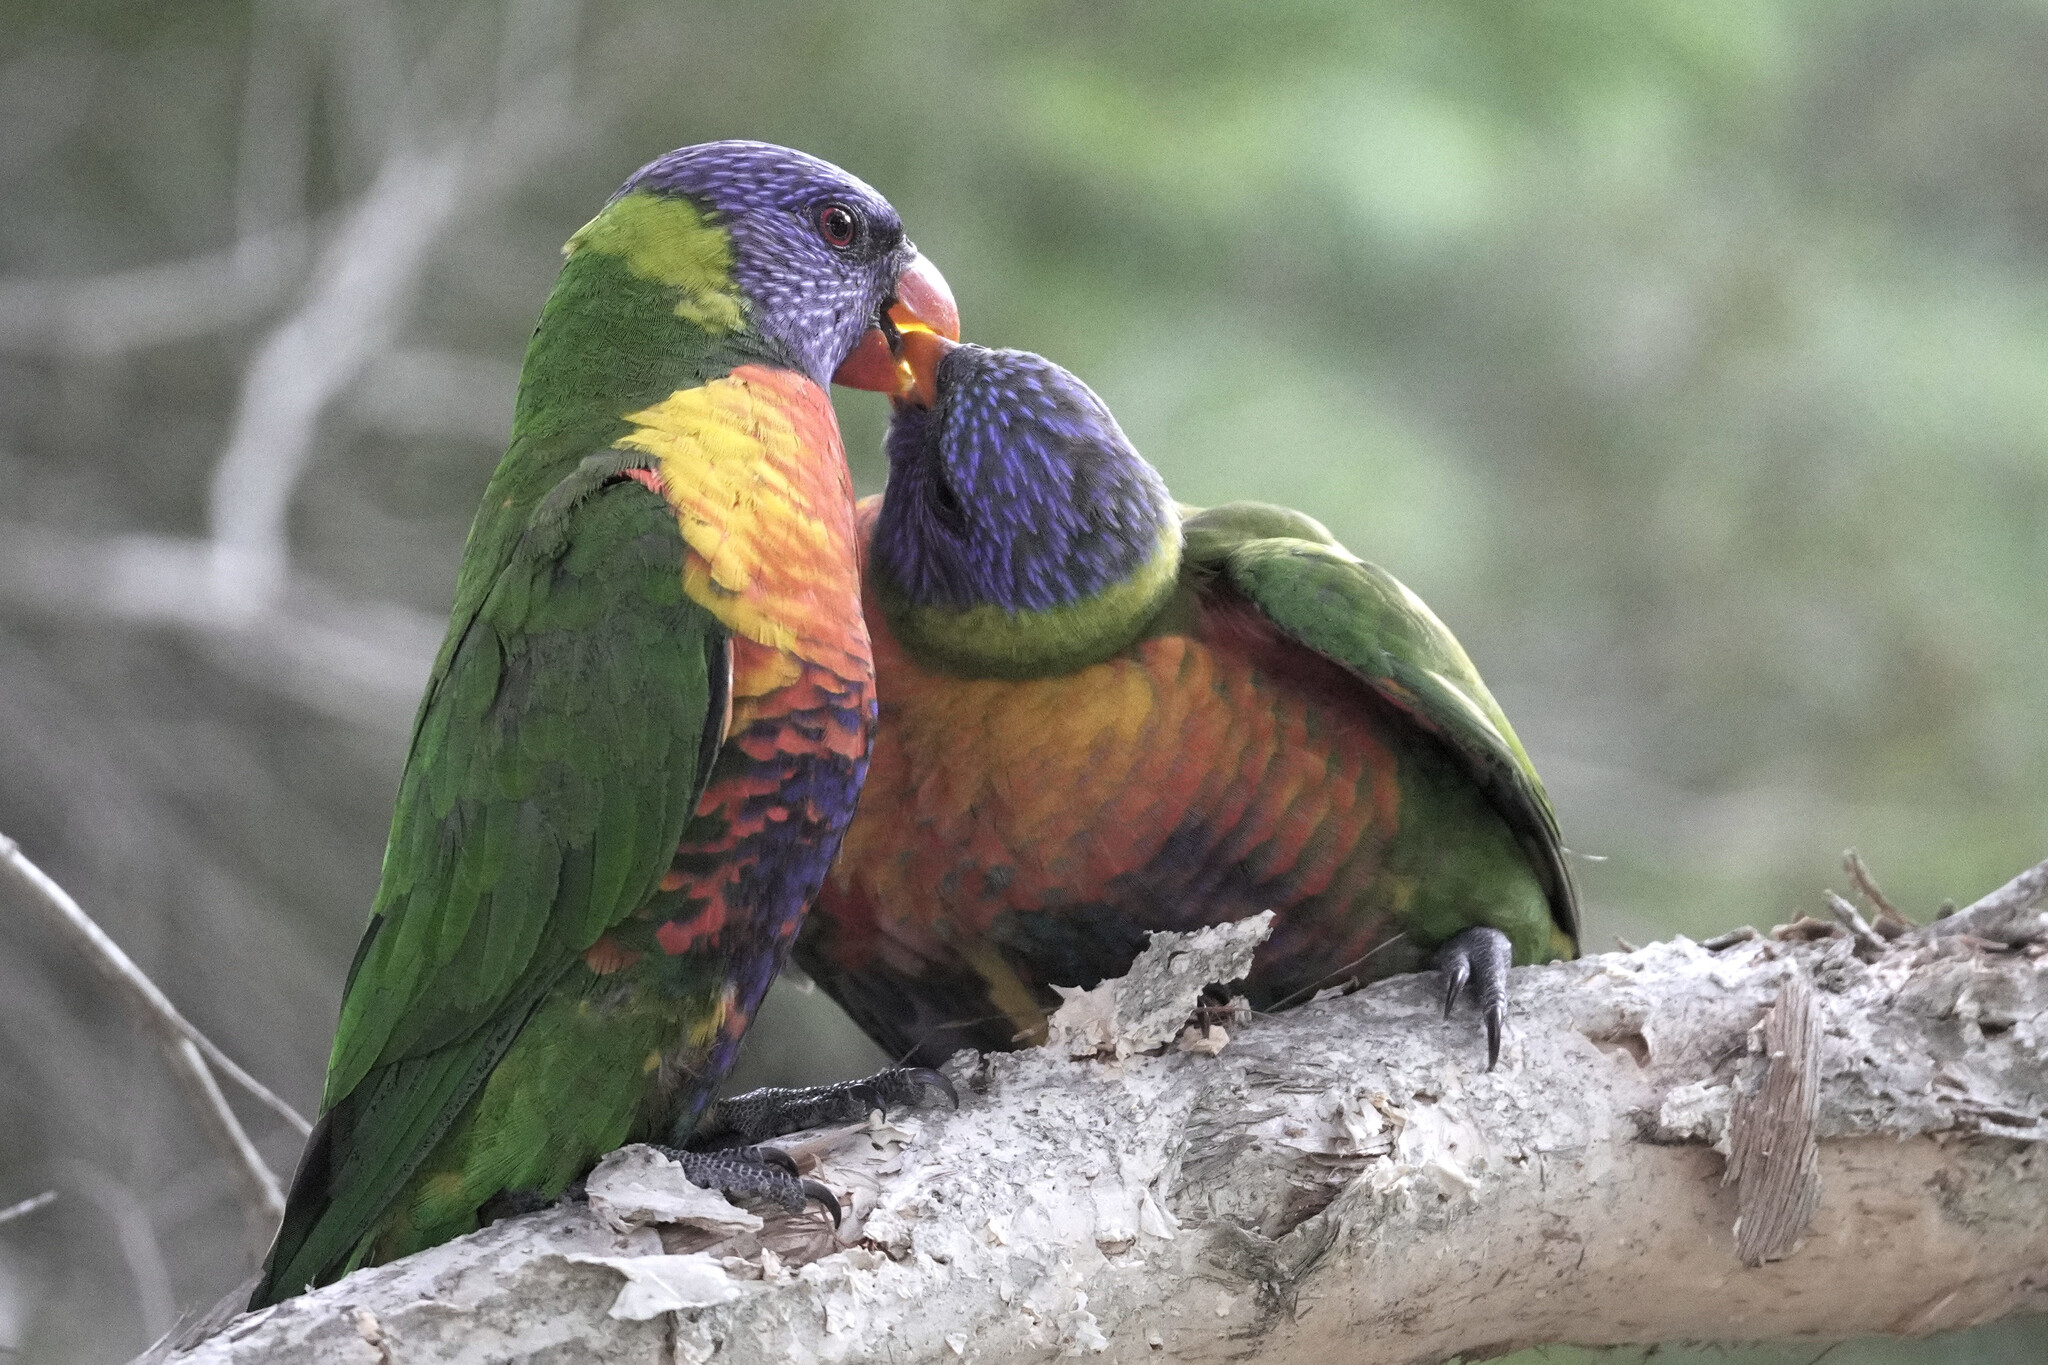
\includegraphics[width=.8\textwidth]{images/L08-sharing.jpg}

Credit: Patrick Lam
\end{center}

\end{frame}

\begin{frame}
\frametitle{Sharing is Caring}

The next idea is sharing: can we use a reader-writer lock to allow much more concurrency than we would get if everything used exclusive locking? 

If there will be a lot of writes then there's limited benefit to this speedup, \\
\hspace*{2em} but if reads are the majority of operations then it is worth doing. 

We can also try to find a way to break a critical section up into two or more smaller ones, if that can be done correctly!

\end{frame}

\begin{frame}
\frametitle{Nevermind, I wanted something else...}

The next idea has to do with changing when (and how) you need the data. 

Shrink the critical section to just pull a copy of the shared data and operate on the shared data. 
 
 
But you saw the earlier discussion about critical section sizes, right? So you did that already...?


\end{frame} 


\begin{frame}[fragile]
\frametitle{Try, Try Again}

The last solution suggested is to use try-lock primitives:

\begin{lstlisting}[language=Rust]
    let mut retries = 0;
    let retries_limit = 10;
    let counter = Mutex::new(0);

    loop {
        if retries < retries_limit {
            let mut l = counter.try_lock();
            if l.is_ok() {
                *l.unwrap() = 1;
                break;
            } else {
                retries = retries + 1;
                thread::yield_now();
            }
        } else {
            *counter.lock().unwrap() = 1;
            break;
        }
    }
}
\end{lstlisting}


If we reach the limit then we just give up and enter the queue!

\end{frame}



\begin{frame}
\frametitle{Polling?!}

It looks like polling for the critical section. 

The limit on the number of tries helps in case the critical section belongs to a low priority thread and we need the current thread to be blocked.

Under this scheme, if $A$ is going to release the critical section, $B$ does not immediately become the owner. 

$A$ may keep running and $A$ might even get the critical section again before $B$ tries again to acquire the lock (and may succeed). 

Even if the spin limit is as low as 2, this means two threads can recover from contention without creating a convoy

\end{frame}


\begin{frame}
\frametitle{You've been... THUNDERSTRUCK!}

\begin{center}
\includegraphics[width=.8\textwidth]{images/L08-thundering-herd.jpg}

Credit: public domain, Famous Players, 1925
\end{center}

\end{frame}


\begin{frame}
\frametitle{You've been... THUNDERSTRUCK!}

The lock convoy has some similarities with a different problem called the \alert{thundering herd problem}. 

In the thundering herd problem, some condition is fulfilled (e.g., broadcast on a condition variable) and it triggers a large number of threads to wake up. 

It is likely they can't all proceed, so some will get blocked and then awoken again all at once in the future. 

In this case it would be better to wake up one thread at a time instead of all of them.

\end{frame}

\begin{frame}
\frametitle{Lost Wakeups}

\begin{center}
\includegraphics[width=.8\textwidth]{images/L08-sleeping-beauty.jpg}

Credit: public domain, John Collier, \emph{Sleeping Beauty}, 1929
\end{center}
\end{frame}

\begin{frame}
\frametitle{Lost Wakeups}


Beware! Waking up one thread at a time only works when threads are identical.

Otherwise, you're better off waking all the threads just in case, to avoid correctness issues.

\end{frame}

\begin{frame}
\frametitle{Locks and Atomics}

 Atomics are a lower-overhead alternative to
locks as long as you're doing suitable operations. 

Sometimes: just want that operations are indivisible.

Key idea: an \alert{atomic operation} is indivisible.\\
\quad Other threads see state before or after the operation; nothing in between.

\end{frame}


%%%%%%%%%%%%%%%%%%%%%%%%%%%%%%%%%%%%%%%%%%%%%%%%%%%%%%%%%%%%%%%%%%%%%%%%%%%%%%%%
\begin{frame}[fragile]
  \frametitle{About Atomics}

\vspace*{-2em}

\Large
    Use the default {\tt Ordering::SeqCst}.\\
    (= sequential consistency)\\[1em]

    \alert{Don't use relaxed atomics unless you're an expert!}\\[1em]
    
    
\end{frame}
%%%%%%%%%%%%%%%%%%%%%%%%%%%%%%%%%%%%%%%%%%%%%%%%%%%%%%%%%%%%%%%%%%%%%%%%%%%%%%%%



%%%%%%%%%%%%%%%%%%%%%%%%%%%%%%%%%%%%%%%%%%%%%%%%%%%%%%%%%%%%%%%%%%%%%%%%%%%%%%%%
\begin{frame}[fragile]
  \frametitle{Really, don't use relaxed atomics!}
  \begin{center}
    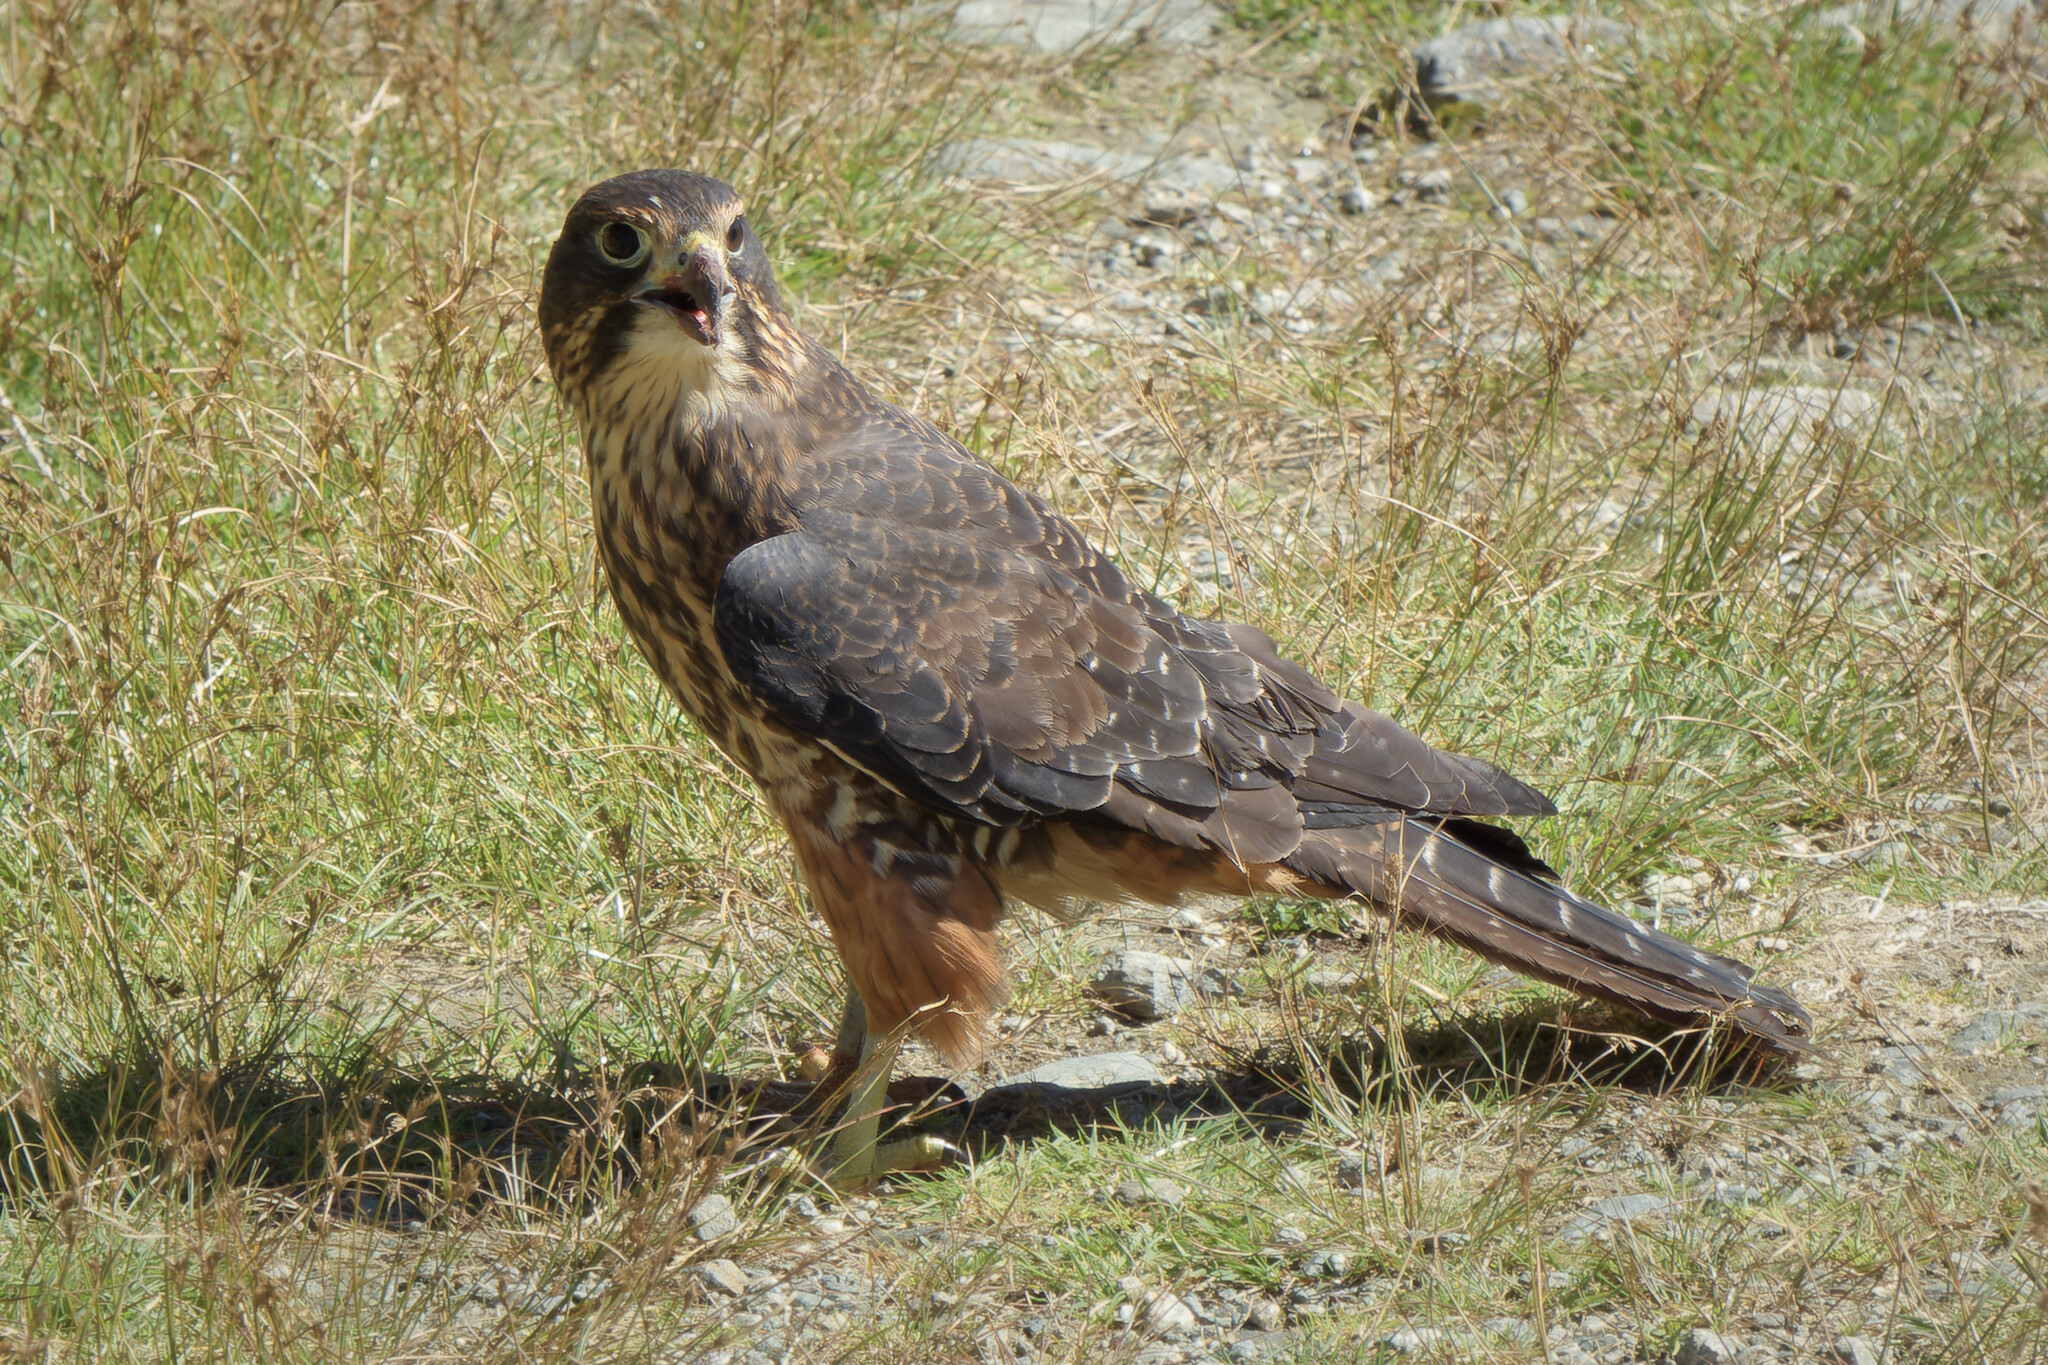
\includegraphics[width=.8\textwidth]{images/disapproving-bird}\\
    Photo: Patrick Lam
  \end{center}
\end{frame}
%%%%%%%%%%%%%%%%%%%%%%%%%%%%%%%%%%%%%%%%%%%%%%%%%%%%%%%%%%%%%%%%%%%%%%%%%%%%%%%%

%%%%%%%%%%%%%%%%%%%%%%%%%%%%%%%%%%%%%%%%%%%%%%%%%%%%%%%%%%%%%%%%%%%%%%%%%%%%%%%%
\begin{frame}[fragile]
  \frametitle{Atomics: Key Idea}
  
    An \emph{atomic operation} is indivisible.\\[1em]
    Other threads see state before or after the operation,
    nothing in between.
  
\end{frame}
%%%%%%%%%%%%%%%%%%%%%%%%%%%%%%%%%%%%%%%%%%%%%%%%%%%%%%%%%%%%%%%%%%%%%%%%%%%%%%%%


\begin{frame}[fragile]
\frametitle{Simple Atomic Example}

\begin{lstlisting}[language=Rust]
use std::sync::atomic::{AtomicBool, Ordering};

fn main() {
   let b = AtomicBool::new(false);
   b.store(true, Ordering::SeqCst);
   println!("{}", b.load(Ordering::SeqCst));
}
\end{lstlisting}

  Reads and writes are straightforward: load and store.

No assignment operator!

\end{frame}


%%%%%%%%%%%%%%%%%%%%%%%%%%%%%%%%%%%%%%%%%%%%%%%%%%%%%%%%%%%%%%%%%%%%%%%%%%%%%%%%
\begin{frame}
  \frametitle{What to do with Atomics}

  

    \Large
    Kinds of operations:
    \begin{itemize}
    \item reads
    \item writes
    \item read-modify-write (RMW)
    \end{itemize}
    
\end{frame}
%%%%%%%%%%%%%%%%%%%%%%%%%%%%%%%%%%%%%%%%%%%%%%%%%%%%%%%%%%%%%%%%%%%%%%%%%%%%%%%%

%%%%%%%%%%%%%%%%%%%%%%%%%%%%%%%%%%%%%%%%%%%%%%%%%%%%%%%%%%%%%%%%%%%%%%%%%%%%%%%%
\begin{frame}
  \frametitle{Read-Modify-Write (RMW)}

  \texttt{fetch\_add} is what you would use to atomically increase the variable's value. 
  
  In C, \texttt{count++} is not atomic; in Rust we would use\\
  \qquad \texttt{count.fetch\_add(1, Ordering::SeqCst)}.

See also: \texttt{fetch\_sub}, \texttt{fetch\_max}, \texttt{fetch\_min}, and the bitwise operations \texttt{and, nand, or, xor}.
  
\end{frame}
%%%%%%%%%%%%%%%%%%%%%%%%%%%%%%%%%%%%%%%%%%%%%%%%%%%%%%%%%%%%%%%%%%%%%%%%%%%%%%%%


\begin{frame}[fragile]
  \frametitle{Compare and Swap}

  
  Also called {\bf compare and exchange} ({\tt cmpxchg} instruction).

  \begin{lstlisting}[language=C]
int compare_and_swap (int* reg, int oldval, int newval) {
  int old_reg_val = *reg;
  if (old_reg_val == oldval) 
     *reg = newval;
  return old_reg_val;
}
  \end{lstlisting}

  \begin{itemize}
    \item Afterwards, you can check if it returned {\tt oldval}.
    \item If it did, you know you changed it.
  \end{itemize}
  
\end{frame}


\begin{frame}
\frametitle{The Rust Equivalent}

The Rust equivalent for this is called \texttt{compare\_and\_swap}

It takes as parameters the expected old value, the desired new value, and the ordering.

We'll see an example in just a moment. 

\end{frame}


\begin{frame}[fragile]
  \frametitle{Implementing a Spinlock}

  
  Use compare-and-swap to implement spinlock:
\begin{lstlisting}[language=Rust]
use std::sync::atomic::{AtomicBool, Ordering, spin_loop_hint};

fn main() {
    let my_lock = AtomicBool::new(false);
    // ... Other stuff happens

    while my_lock.compare_and_swap(false, true, Ordering::SeqCst) == true {
	// The lock was `true`, someone else had the lock, so try again
        spin_loop_hint();
    }
    // Inside critical section
    my_lock.store(false, Ordering::SeqCst);
}
  \end{lstlisting}

\end{frame}


\begin{frame}[fragile]
  \frametitle{ABA Problem}

  
    Sometimes you'll read a location twice.\\[1em]

    If the value is the same, nothing has changed, right?

    \pause

    \alert{No.} This is an {\bf ABA problem}.\\[1em]

    You can combat this by ``tagging'': modify value with nonce upon each write.\\[1em]

    Can keep value separately from nonce; double compare and swap atomically swaps both value and nonce.\\[2em]


  
\end{frame}
%%%%%%%%%%%%%%%%%%%%%%%%%%%%%%%%%%%%%%%%%%%%%%%%%%%%%%%%%%%%%%%%%%%%%%%%%%%%%%%%


\begin{frame}
\frametitle{Waterloo...}

\begin{center}
	\includegraphics[width=0.7\textwidth]{images/abba.jpeg}
\end{center}

The ABA problem is not any sort of acronym nor a reference to this: \url{https://www.youtube.com/watch?v=Sj_9CiNkkn4}


\end{frame}



\begin{frame}
\frametitle{ABA}

It's a value that is A, then changed to B, then changed back to A. 

The ABA problem is a big mess for the designer of lock-free Compare-And-Swap routines. 

\begin{enumerate}
	\item $P_{1}$ reads $A_{i}$ from location $L_{i}$.
	\item $P_{k}$ interrupts $P_{1}$; $P_{k}$ stores the value $B$ into $L_{i}$.
	\item $P_{j}$ stores the value $A_{i}$ into $L_{i}$.
	\item $P_{1}$ resumes; it executes a false positive CAS.
\end{enumerate} 


\end{frame}



\begin{frame}
\frametitle{False Positive}

It's a ``false positive'' because $P_{1}$'s compare-and-swap operation succeeds even though the value at $L_{i}$ has been modified in the meantime. 

If this doesn't seem like a bad thing, consider this. 

If you have a data structure that will be accessed by multiple threads, you might be controlling access to it by the compare-and-swap routine. 

What should happen is the algorithm should keep trying until the data structure in question has not been modified by any other thread in the meantime. 

But with a false positive we get the impression that things didn't change, even though they really did.

\end{frame}



\begin{frame}
\frametitle{Napoleon was defeated...}

You can combat this by ``tagging'': modify value with nonce upon each
write.  

You can also keep the value separately from the nonce; double
compare and swap atomically swaps both value and nonce.

Another example of this: Java \texttt{ConcurrentModificationException} is detected by checking the modification count of a collection.

\end{frame}


\begin{frame}
\frametitle{Ask your doctor if atomics are right for you!}

Race conditions can still happen if threads are not properly coordinated.

Unfortunately, not every atomic operation is portable. 

Rust will try its best to give you the atomic types that you ask for.

\end{frame}


%%%%%%%%%%%%%%%%%%%%%%%%%%%%%%%%%%%%%%%%%%%%%%%%%%%%%%%%%%%%%%%%%%%%%%%%%%%%%%%%

\begin{frame}
\frametitle{Do Free Lunches Exist?}

\begin{center}
\includegraphics[width=0.6\textwidth]{images/freelunch.jpg}
\end{center}

\end{frame}


\begin{frame}
\frametitle{Lock Freedom}

Suppose we'd like to operate in a world in which there are no locks. 

Research has gone into the idea of lock-free data structures. 

If you have a map and it will be shared between threads, the normal thing would be to protect access to the map with a mutex (lock). 

But what if the data structure was written in such a way that we didn't have to do that? 

That would be a lock-free data structure.

\end{frame}

\begin{frame}
\frametitle{Use Locks Wisely!}

\begin{center}
	\includegraphics[width=0.5\textwidth]{images/usebombswisely.png}
\end{center}

Often, normal locking and unlocking behaviour is sufficient.

\end{frame}

\begin{frame}
\frametitle{Use Locks Wisely!}


We likely want to use it when we need to guarantee that progress is made. 

Or: when we really can't use locks (e.g., signal handler), or where a thread dying while holding a lock results in the whole system hanging.

\end{frame}

\begin{frame}
\frametitle{Non-Blocking Data Structure}

Non-blocking data struct: one where no operation can result in being blocked. 


\begin{center}
	\includegraphics[width=0.5\textwidth]{images/noblocks.jpg}
\end{center}


\end{frame}

\begin{frame}
\frametitle{Non-Blocking Data Structure}

Java has concurrency-controlled data structures in which locking and unlocking is handled for you, but those can still be blocking. 

Lock-free data structures are always inherently non-blocking. 

A spin lock or busy-waiting approach is not lock-free, because if the thread holding the lock is suspended then everyone else is stuck!

\end{frame}

\begin{frame}
\frametitle{Lock-Free Data Structure}
A lock-free data structure doesn't use any locks (duh) but there's also some implication that this is also thread-safe.

You can't make all your data structures lock-free ones by just deleting all the mutex code (sorry). 

Lock-free also doesn't mean it's a free-for-all; there can be restrictions. 

For example, a queue may allow one thread to append to the end while another removes from the front, but not 2 removals at the same time.
\end{frame}



\begin{frame}
\frametitle{Lock-Free Data Structure}

The actual definition of lock-free is more formal. 

If any thread performing an operation gets suspended during the operation, other threads accessing the data structure are still able to complete their tasks.

This is distinct from the idea of waiting, though; an operation might still have to wait its turn or might get restarted.

\end{frame}



\begin{frame}
\frametitle{Wait-Free Data Structures}

You might need wait-free data structures. 

This does not mean that nothing ever has to wait! 

\end{frame}



\begin{frame}
\frametitle{Wait-Free Data Structures}


It does mean that each thread trying to perform some operation will complete it within a bounded number of steps regardless of what any other threads do. 

This means that a compare-and-swap routine with infinite retries is not wait free, because a very unlucky thread could potentially take infinite tries...

The wait free data structures tend to be very complicated...

\end{frame}


\begin{frame}[fragile]
\frametitle{Example Lock-Free Algorithm}

\begin{lstlisting}[language=Rust]
use std::ptr::{self, null_mut};
use std::sync::atomic::{AtomicPtr, Ordering};

pub struct Stack<T> {
    head: AtomicPtr<Node<T>>,
}

struct Node<T> {
    data: T,
    next: *mut Node<T>,
}

impl<T> Stack<T> {
    pub fn new() -> Stack<T> {
        Stack {
            head: AtomicPtr::new(null_mut()),
        }
    }
}
\end{lstlisting}
\end{frame}


\begin{frame}[fragile]
\frametitle{Example Lock-Free Algorithm}

\begin{lstlisting}[language=Rust]
impl<T> Stack<T> {
    pub fn push(&self, t: T) {
        // allocate the node, and immediately turn it into a *mut pointer
        let n = Box::into_raw(Box::new(Node {
            data: t,
            next: null_mut(),
        }));
        loop {
            // snapshot current head
            let head = self.head.load(Ordering::SeqCst);

            // update `next` pointer with snapshot
            unsafe { (*n).next = head; }

            // if snapshot is still good, link in new node
            if self.head.compare_and_swap(head, n, Ordering::SeqCst) == head {
                break
            }
        }
    }
}
\end{lstlisting}


\end{frame}

\begin{frame}[fragile]
\frametitle{Example Wait-Free Algorithm}

\begin{lstlisting}[language=Rust]
fn increment_counter(ctr: &AtomicI32) {
    ctr.fetch_add(1, Ordering::SeqCst);
}

fn decrement_counter(ctr: &AtomicI32) {
    let old = ctr.fetch_sub(1, Ordering::SeqCst);
    if old == 1 { // We just decremented from 1 to 0
        println!{ "All done." }
    }
}
\end{lstlisting}


\end{frame}


\begin{frame}
\frametitle{To Lock Free, or Not to Lock Free}

Are lock-free programming techniques somehow better for performance? Maybe!

Lock-free algorithms are about ensuring there is forward progress in the system and not really specifically about speed. 

A particular algorithm implementation might be faster under lock-free algorithms.

But often they are not. In fact, the lock-free algorithms could be slower, in which case you use them because you must, not because it is particularly speedy.

\end{frame}


\end{document}

